\chapter{Исследовательский раздел}\label{sec:exp}

В данном разделе будут представлены замеры времени работы реализаций алгоритмов.

\section{Технические характеристики}

Технические характеристики устройства, на котором выполнялось тестирование представлены далее.

\begin{itemize}
    \item Операционная система: macOS Catalina версия 10.15.6;
    \item Память: 8 GB 1600 MHz DDR3;
    \item Процессор: 1,8 GHz 2‑ядерный процессор Intel Core i5.
\end{itemize}

Тестирование проводилось на ноутбуке, включенном в сеть электропитания.
Во время тестирования ноутбук был нагружен только встроенными приложениями окружения рабочего стола.

\section{Сравнительный анализ на основе замеров времени работы алгоритмов}

Был проведен замер времени работы каждого из алгоритмов с помощью функции process\_time(), которая находится в модуле time языка Python.
Замеры времени усреднялись, для каждого алгоритма проводилось по 20 итераций.

\begin{table}[H]
	\begin{center}
	    \captionsetup{singlelinecheck = false, justification=centering}
		\caption{Результаты замеров времени}
		\begin{tabular}{c|c|c|c|c}
			Длина & Рек. Лев. & Кэш. Лев & Рек. Д.-Лев. & Кэш. Д.-Лев\\
			\hline
1 & 2.72E-06 & 5.10E-06 & 2.44E-06 & 9.83E-06\\
2 & 1.17E-05 & 8.75E-06 & 1.25E-05 & 1.56E-05\\
3 & 5.53E-05 & 1.43E-05 & 7.31E-05 & 2.88E-05\\
4 & 2.65E-04 & 2.45E-05 & 2.93E-04 & 4.04E-05\\
5 & 1.51E-03 & 4.60E-05 & 1.74E-03 & 5.23E-05\\
6 & 8.55E-03 & 4.91E-05 & 8.93E-03 & 5.03E-05\\
7 & 4.35E-02 & 5.51E-05 & 4.77E-02 & 6.28E-05\\
8 & 2.43E-01 & 7.07E-05 & 2.63E-01 & 8.40E-05\\
9 & 1.36E+00 & 9.78E-05 & 1.46E+00 & 1.21E-04\\
10 & - & 1.09E-04 & - & 1.30E-04\\
20 & - & 4.82E-04 & - & 5.82E-04\\
30 & - & 9.28E-04 & - & 1.33E-03\\
50 & - & 2.49E-03 & - & 3.87E-03\\
100 & - & 1.02E-02 & - & 1.21E-02\\
200 & - & 3.98E-02 & - & 4.93E-02\\
		\end{tabular}
	\end{center}
\end{table}

\begin{figure}[H]
	\centering
	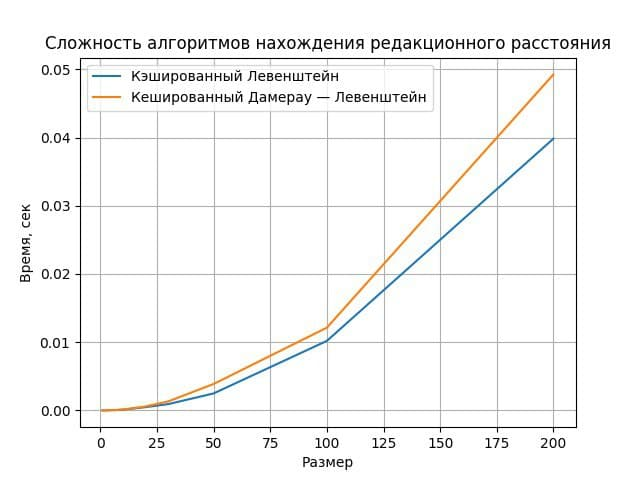
\includegraphics[scale = 0.7]{assets/cacheGraph.jpg}
	\caption{Сравнение времени работы кеширующих алгоритмов поиска расстояния Левенштейна и Дамерау-Левенштейна}
	\label{fig:plot_sorted}
\end{figure}

\begin{figure}[H]
	\centering
	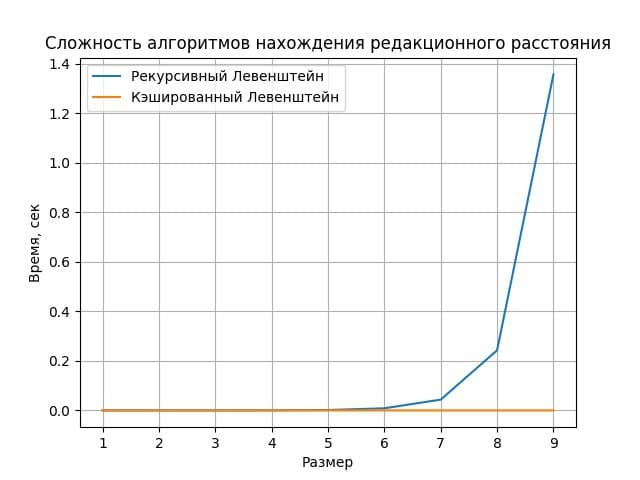
\includegraphics[scale = 0.7]{assets/levGraph.jpg}
	\caption{Сравнение времени работы рекурсивной и кеширующей реализаций алгоритма Левенштейна}
	\label{fig:plot_sorted}
\end{figure}

\section{Вывод}

В данном разделе было произведено сравнение количества затраченного времени вышеизложенных алгоритмов.

Исходя из полученных результатов, можно сделать вывод, что при длинах строк менее 30 символов разница по времени между кеширующими реализациями незначительна, однако при увеличении длины строки алгоритм поиска расстояния Левенштейна оказывается быстрее на 20\% (при длинах строк равных 200).
Это обосновывается тем, что у алгоритма поиска расстояния Дамерау-Левенштейна задействуется дополнительная операция, которая замедляет алгоритм. Также можно сделать вывод, что рекурсивный алгоритм становится менее эффективным, чем кеширующий.
Из этого можно сделать вывод о том, что при малых длинах строк (1–5 символов) предпочтительнее использовать рекурсивные алгоритмы, однако при обработке более длинных
строк (болеее 5 символов) кеширующие алгоритмы оказываются многократно более эффективными и рекомендуются к использованию.